In lab 2 we made storage elements and bus of the Chacc processor. The storage
elements (Regsiter and memory) were made using generics, this way we could use
the same storage elements in many different places of our processor later on.
\subsection*{Storage elements, Register and Memory}
The register was built using one generic value, \textbf{W}, which was used to
determine width of the data stored in the register. The register was implemented
using a process which was sensetive to \textbf{CLK} and \textbf{ARESETN}.
Whenever \textbf{ARESETN} is active (=0) the output from the register is changed
to 0. If we are on a rising \textbf{CLK} edge and \textbf{LOAD\_ENABLE} is
turned on then we set the output to whatever is in the input. If none of those
two conditions are fulfilled we keep the output as it is.

The memory was built very similarly to the register with a few key differences.
The first is that two generics where used \textbf{DATA\_WIDTH} and
\textbf{ADRESS\_WIDTH}. These generics were used to make a new type
\textbf{MEMORY\_ARRAY}, which is an array of $2^{\textbf{ADDRES\_WIDTH}}$
entries of a \\ \textbf{DATA\_WIDTH} wide STD\_LOGIC\_VECTOR. This array can also
be initialized by a function \textbf{init\_memory\_wfile}. The generics were
also used to specify the width of the adress and data inputs as well as the
output from the memory.
\subsection*{The bus}
The bus has 4 enable signals from the different parts of the processor that want
to use it. We need to enable only one of them to get actual access to the bus.
We did this by concatenating the select signals into one combined signal and
then, using a with select statement, choosing the signal that is connected to
the bus. If more than one select signal, or no select signal is used we instead
set all the bits on the bus to zero.
\subsection*{Waveform}
In figure \ref{lab2:waveform} the waveform for the different signals of a 
register is shown. Showing that it works as expected.
\begin{figure}
  \caption{Waveform showing the correct functionality of the register.}
  \label{lab2:waveform}
  \centering
  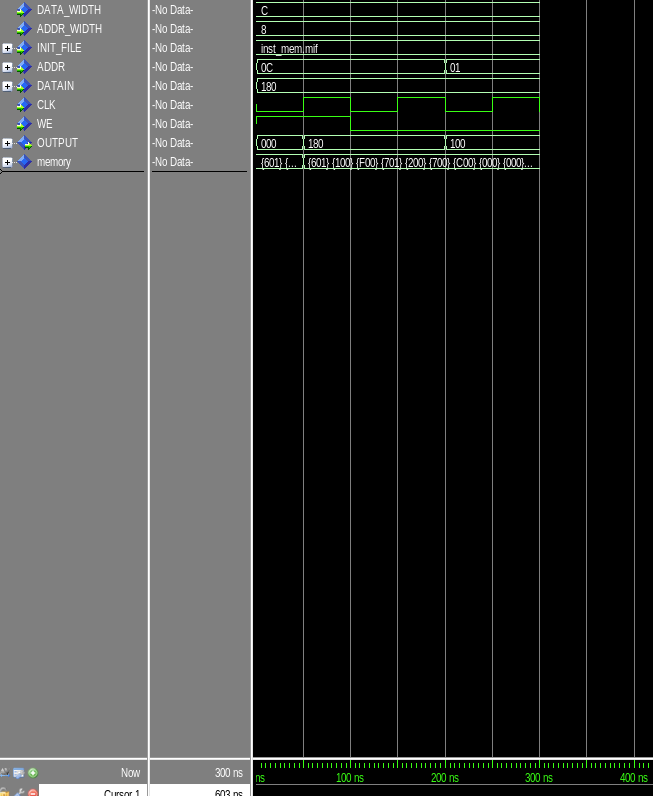
\includegraphics[width=\textwidth]{lab2-waveform.png}
\end{figure}
